%%%%%%%%%%%%%%%%%%%%%%%%%%%%%%%%%%%%%%%%%%%%%%%%%%%%%%%%%%%%%%%%%%%%%%%%%%%%%%%%
%% Plantilla de memoria en LaTeX para la EIF - Universidad Rey Juan Carlos
%%
%% Por Gregorio Robles <grex arroba gsyc.urjc.es>
%%     Grupo de Sistemas y Comunicaciones
%%     Escuela de Ingeniería de Fuenlabrada
%%     Universidad Rey Juan Carlos
%% (muchas ideas tomadas de Internet, colegas del GSyC, antiguos alumnos...
%%  etc. Muchas gracias a todos)
%%
%% La última versión de esta plantilla está siempre disponible en:
%%     https://github.com/gregoriorobles/plantilla-memoria
%%
%% Para obtener PDF, ejecuta en la shell:
%%   make
%% (las imágenes deben ir en PNG o JPG)

%%%%%%%%%%%%%%%%%%%%%%%%%%%%%%%%%%%%%%%%%%%%%%%%%%%%%%%%%%%%%%%%%%%%%%%%%%%%%%%%

\documentclass[a4paper, 12pt]{book}
%\usepackage[T1]{fontenc}

\usepackage[a4paper, left=2.5cm, right=2.5cm, top=3cm, bottom=3cm]{geometry}
\usepackage{times}
\usepackage[utf8]{inputenc}
\usepackage[spanish]{babel} % Comenta esta línea si tu memoria es en inglés
\usepackage{url}
%\usepackage[dvipdfm]{graphicx}
\usepackage{graphicx}
\usepackage{float}  %% H para posicionar figuras
\usepackage[nottoc, notlot, notlof, notindex]{tocbibind} %% Opciones de índice
\usepackage{latexsym}  %% Logo LaTeX

\title{Memoria del Proyecto}
\author{Nombre del autor}

\renewcommand{\baselinestretch}{1.5}  %% Interlineado

\begin{document}

\renewcommand{\refname}{Bibliografía}  %% Renombrando
\renewcommand{\appendixname}{Apéndice}


%%%%%%%%%%%%%%%%%%%%%%%%%%%%%%%%%%%%%%%%%%%%%%%%%%%%%%%%%%%%%%%%%%%%%%%%%%%%%%%%
% PORTADA

\begin{titlepage}
\begin{center}
\includegraphics[scale=0.6]{img/URJ_logo_Color_POS.png}

\vspace{1.75cm}

\LARGE
ESCUELA DE INGENIERÍA DE FUENLABRADA
\vspace{1cm}

\LARGE
GRADO EN INGENIERIA EN SISTEMAS AUDIOVISUALES Y MULTIMEDIA

\vspace{1cm}
\LARGE
\textbf{TRABAJO FIN DE GRADO}

\vspace{2cm}

\Large
ENTORNO INMERSIVO 3D CON TECNOLOGÍAS WEB

\vspace{2cm}

\large
Autor : Jorge Luis Grande González \\
Tutor : Dr. Gregorio Robles\\
\vspace{1cm}

\large
Curso académico 2023/2024

\end{center}
\end{titlepage}

\newpage
\mbox{}
\thispagestyle{empty} % para que no se numere esta pagina



%%%%%%%%%%%%%%%%%%%%%%%%%%%%%%%%%%%%%%%%%%%%%%%%%%%%%%%%%%%%%%%%%%%%%%%%%%%%%%%%
%%%% Para firmar
\clearpage
\pagenumbering{gobble}
\chapter*{}

\vspace{-4cm}
\begin{center}
\LARGE
\textbf{Trabajo Fin de Grado/Máster}

\vspace{1cm}
\large
Entorno Inmersivo 3D con Tecnologías Web

\vspace{1cm}
\large
\textbf{Autor :} Jorge Luis Grande González \\
\textbf{Tutor :} Dr. Gregorio Robles

\end{center}

\vspace{1cm}
La defensa del presente Proyecto Fin de Carrera se realizó el día \qquad$\;\,$ de \qquad\qquad\qquad\qquad \newline de 2024, siendo calificada por el siguiente tribunal:


\vspace{0.5cm}
\textbf{Presidente:}

\vspace{1.2cm}
\textbf{Secretario:}

\vspace{1.2cm}
\textbf{Vocal:}


\vspace{1.2cm}
y habiendo obtenido la siguiente calificación:

\vspace{1cm}
\textbf{Calificación:}


\vspace{1cm}
\begin{flushright}
Fuenlabrada, a \qquad$\;\,$ de \qquad\qquad\qquad\qquad de 2024
\end{flushright}

%%%%%%%%%%%%%%%%%%%%%%%%%%%%%%%%%%%%%%%%%%%%%%%%%%%%%%%%%%%%%%%%%%%%%%%%%%%%%%%%
%%%% Dedicatoria

\chapter*{}
\pagenumbering{Roman} % para comenzar la numeracion de paginas en numeros romanos
\begin{flushright}
\textit{Dedicado a \\
mi madre}
\end{flushright}

%%%%%%%%%%%%%%%%%%%%%%%%%%%%%%%%%%%%%%%%%%%%%%%%%%%%%%%%%%%%%%%%%%%%%%%%%%%%%%%%
%%%% Agradecimientos

\chapter*{Agradecimientos}
%\addcontentsline{toc}{chapter}{Agradecimientos} % si queremos que aparezca en el índice
\markboth{AGRADECIMIENTOS}{AGRADECIMIENTOS} % encabezado 

Aquí vienen los agradecimientos\ldots Aunque está bien acordarse de la pareja, no hay que olvidarse de dar las gracias a tu madre, que aunque a veces no lo parezca disfrutará tanto de tus logros como tú\ldots 
Además, la pareja quizás no sea para siempre, pero tu madre sí.

%%%%%%%%%%%%%%%%%%%%%%%%%%%%%%%%%%%%%%%%%%%%%%%%%%%%%%%%%%%%%%%%%%%%%%%%%%%%%%%%
%%%% Resumen

\chapter*{Resumen}
%\addcontentsline{toc}{chapter}{Resumen} % si queremos que aparezca en el índice
\markboth{RESUMEN}{RESUMEN} % encabezado

Este proyecto se enfoca en el desarrollo de un sistema de comunicación interactiva implementado en un entorno de realidad virtual, 
utilizando el Protocolo de Inicio de Sesión (SIP) y el Protocolo de Transporte en Tiempo Real (RTP) para gestionar la señalización y 
la transmisión de datos multimedia. El objetivo principal es construir una representación visual y funcional que permita a los usuarios 
experimentar de manera tangible los flujos y la gestión de las comunicaciones en tiempo real, utilizando tecnologías de realidad virtual.

\bigskip

Para lograr este objetivo, se ha utilizado una combinación de herramientas y tecnologías avanzadas, incluyendo la biblioteca de 
JavaScript Three.js para la renderización de gráficos 3D, así como varios módulos adicionales de Three.js que apoyan la interactividad en 
entornos VR como VRButton.js, XRControllerModelFactory.js, Stats.js, y OrbitControls.js. El desarrollo se ha llevado a cabo dentro del marco 
de un proyecto educativo en la universidad, buscando proporcionar una herramienta de enseñanza para 
estudiantes interesados en la realidad virtual y las telecomunicaciones.

\bigskip

Este TFG se sitúa en el contexto de la necesidad creciente de soluciones tecnológicas avanzadas en el campo de las comunicaciones y 
la educación virtual. Con el uso de la realidad virtual, el proyecto no solo demuestra la viabilidad técnica de simular sistemas de comunicación 
complejos en un entorno inmersivo, sino que también explora nuevas posibilidades para la enseñanza y el aprendizaje de conceptos 
avanzados de telecomunicaciones.

\bigskip

En resumen, este trabajo aporta a la comprensión de cómo las tecnologías emergentes pueden ser aplicadas para mejorar los sistemas de comunicación digital y 
ofrece una base sólida para futuras investigaciones en la aplicación de la realidad virtual en educación y comunicaciones.


%%%%%%%%%%%%%%%%%%%%%%%%%%%%%%%%%%%%%%%%%%%%%%%%%%%%%%%%%%%%%%%%%%%%%%%%%%%%%%%%
%%%% Resumen en inglés

\chapter*{Summary}
%\addcontentsline{toc}{chapter}{Summary} % si queremos que aparezca en el índice
\markboth{SUMMARY}{SUMMARY} % encabezado

This project focuses on the development of an interactive communication system implemented in a virtual reality environment, 
utilizing the Session Initiation Protocol (SIP) and the Real-time Transport Protocol (RTP) to manage signaling and multimedia data transmission. 
The main goal is to construct a visual and functional representation that allows users to tangibly experience the flows and 
management of communications in real-time, using virtual reality technologies.

\bigskip

To achieve this objective, a combination of advanced tools and technologies has been used, including the JavaScript library Three.js for 3D graphics rendering, 
as well as several additional Three.js modules that support interactivity in VR environments such as VRButton.js, XRControllerModelFactory.js, Stats.js, 
and OrbitControls.js. The development has been carried out within the framework of an educational project at the university, aiming to provide a teaching tool 
for students interested in virtual reality and telecommunications.

\bigskip

This thesis is situated in the context of the growing need for advanced technological solutions in the field of communications and virtual education. 
With the use of virtual reality, the project not only demonstrates the technical feasibility of simulating complex communication systems in an immersive 
environment but also explores new possibilities for teaching and learning advanced telecommunications concepts.

\bigskip

In summary, this work contributes to the understanding of how emerging technologies can be applied to enhance digital communication systems and provides a solid 
foundation for future research in the application of virtual reality in education and communications.

%%%%%%%%%%%%%%%%%%%%%%%%%%%%%%%%%%%%%%%%%%%%%%%%%%%%%%%%%%%%%%%%%%%%%%%%%%%%%%%%
%%%%%%%%%%%%%%%%%%%%%%%%%%%%%%%%%%%%%%%%%%%%%%%%%%%%%%%%%%%%%%%%%%%%%%%%%%%%%%%%
% ÍNDICES %
%%%%%%%%%%%%%%%%%%%%%%%%%%%%%%%%%%%%%%%%%%%%%%%%%%%%%%%%%%%%%%%%%%%%%%%%%%%%%%%%

% Las buenas noticias es que los índices se generan automáticamente.
% Lo único que tienes que hacer es elegir cuáles quieren que se generen,
% y comentar/descomentar esa instrucción de LaTeX.

%%%% Índice de contenidos
\tableofcontents 
%%%% Índice de figuras
\cleardoublepage
%\addcontentsline{toc}{chapter}{Lista de figuras} % para que aparezca en el indice de contenidos
\listoffigures % indice de figuras
%%%% Índice de tablas
%\cleardoublepage
%\addcontentsline{toc}{chapter}{Lista de tablas} % para que aparezca en el indice de contenidos
%\listoftables % indice de tablas


%%%%%%%%%%%%%%%%%%%%%%%%%%%%%%%%%%%%%%%%%%%%%%%%%%%%%%%%%%%%%%%%%%%%%%%%%%%%%%%%
%%%%%%%%%%%%%%%%%%%%%%%%%%%%%%%%%%%%%%%%%%%%%%%%%%%%%%%%%%%%%%%%%%%%%%%%%%%%%%%%
% INTRODUCCIÓN %
%%%%%%%%%%%%%%%%%%%%%%%%%%%%%%%%%%%%%%%%%%%%%%%%%%%%%%%%%%%%%%%%%%%%%%%%%%%%%%%%

\cleardoublepage
\chapter{Introducción}
\label{sec:intro} % etiqueta para poder referenciar luego en el texto con ~\ref{sec:intro}
\pagenumbering{arabic} % para empezar la numeración de página con números
En la era de la transformación digital, las comunicaciones interactivas han evolucionado significativamente, 
incorporando tecnologías inmersivas como la realidad virtual (RV) para ofrecer experiencias más enriquecedoras y colaborativas. 

\bigskip

Este Trabajo de Fin de Grado se centra en el desarrollo e implementación de un sistema de comunicación dentro de un entorno de realidad virtual, 
destacando la aplicación práctica y la comprensión de los protocolos de comunicación estándar, 
como el Protocolo de Inicio de Sesión (SIP) y el Protocolo de Transporte en Tiempo Real (RTP).

\bigskip

La motivación detrás de este proyecto surge de la necesidad de comprender mejor las complejidades de la señalización y 
el manejo de medios en las comunicaciones actuales, y cómo estas pueden ser simuladas y visualizadas en un entorno de realidad virtual. 
A través de la creación de un modelo interactivo, este trabajo pretende proporcionar una herramienta educativa y un medio de 
investigación que permita a los usuarios experimentar de manera tangible el flujo y la gestión de los datos de comunicación.

\bigskip

Con el uso de la realidad virtual, se espera no solo proporcionar una comprensión más profunda de estos protocolos sino también explorar 
las posibilidades que la realidad virtual tiene para ofrecer en términos de aprendizaje interactivo y simulación.


\section{Estructura de la memoria}
\label{sec:estructura}
Esta sección describe la estructura organizativa de la memoria, proporcionando una visión 
general de cada uno de los capítulos principales que componen este trabajo de fin de grado. 
La estructura está diseñada para desarrollar gradualmente el tema, desde la introducción y 
los fundamentos teóricos hasta la implementación práctica y la evaluación de los resultados.

\begin{itemize}
  \item \textbf{Capítulo 1: Introducción} - Se presenta una introducción general al proyecto, estableciendo el contexto y 
  la motivación del estudio.
  
  \item \textbf{Capítulo~\ref{chap:objetivos}: Objetivos} - Detalla los objetivos generales y específicos que guían el desarrollo del proyecto.
  
  \item \textbf{Capítulo~\ref{chap:estado}: Estado del Arte} - Se comentan todas las tecnologías, herramientas y accesorios necesarios
 para el desarrollo y funcionamiento de este proyecto.
  
  \item \textbf{Capítulo~\ref{chap:diseno}: Diseño e implementación} - Describe los métodos utilizados para desarrollar el sistema de comunicación, 
  incluyendo el diseño, las herramientas y tecnologías empleadas.
  
  \item \textbf{Capítulo~\ref{chap:resultados}: Resultados} - Presenta los resultados obtenidos a través de la implementación del sistema.
  
  \item \textbf{Capítulo~\ref{chap:conclusiones}: Conclusiones} - Ofrece un desarrollo de las conclusiones extraídas y 
  las recomendaciones para investigaciones futuras.
\end{itemize}

Cada capítulo está diseñado para construir sobre la información presentada en los anteriores, asegurando un 
flujo lógico y coherente a lo largo de la memoria.




%%%%%%%%%%%%%%%%%%%%%%%%%%%%%%%%%%%%%%%%%%%%%%%%%%%%%%%%%%%%%%%%%%%%%%%%%%%%%%%%
%%%%%%%%%%%%%%%%%%%%%%%%%%%%%%%%%%%%%%%%%%%%%%%%%%%%%%%%%%%%%%%%%%%%%%%%%%%%%%%%
% OBJETIVOS %
%%%%%%%%%%%%%%%%%%%%%%%%%%%%%%%%%%%%%%%%%%%%%%%%%%%%%%%%%%%%%%%%%%%%%%%%%%%%%%%%

\cleardoublepage % empezamos en página impar
\chapter{Objetivos} % título del capítulo (se muestra)
\label{chap:objetivos} % identificador del capítulo (no se muestra, es para poder referenciarlo)

\section{Objetivo general} % título de sección (se muestra)
\label{sec:objetivo-general} % identificador de sección (no se muestra, es para poder referenciarla)

El objetivo principal es construir una representación visual y funcional de los flujos de señalización y 
datos utilizando la biblioteca de JavaScript Three.js, junto con tecnologías de RV para facilitar la interacción con la simulación. 
Se busca demostrar cómo se inicia, se mantiene y se termina una sesión de comunicación, siguiendo los estándares del protocolo SIP, 
y cómo los paquetes RTP son utilizados para el intercambio efectivo de datos multimedia.


\section{Objetivos específicos}
\label{sec:objetivos-especificos}
Para cumplir con el objetivo general de desarrollar una representación visual y funcional de los flujos de señalización 
y datos en un entorno de realidad virtual, se establecen los siguientes objetivos específicos:

\begin{enumerate}
\item Diseñar e implementar un modelo virtual en 3D que simule el entorno de una red de comunicaciones, empleando la biblioteca Three.js.
\item Integrar tecnologías de realidad virtual para facilitar una experiencia inmersiva y 
la interacción del usuario con el modelo de simulación.
\item Desarrollar una interfaz de usuario que permita la visualización y manipulación de los procesos de 
señalización y transmisión de datos, acorde con el protocolo SIP.
\item Implementar la lógica para simular el flujo de mensajes SIP, incluyendo el registro de usuarios, la iniciación y 
recepción de llamadas.
\item Simular la transmisión de datos multimedia a través de paquetes RTP, mostrando la secuencia de envío y recepción en tiempo real.
\item Crear un sistema de retroalimentación visual que indique el estado de las comunicaciones, incluyendo errores y mensajes de confirmación.
\end{enumerate}


%%%%%%%%%%%%%%%%%%%%%%%%%%%%%%%%%%%%%%%%%%%%%%%%%%%%%%%%%%%%%%%%%%%%%%%%%%%%%%%%
%%%%%%%%%%%%%%%%%%%%%%%%%%%%%%%%%%%%%%%%%%%%%%%%%%%%%%%%%%%%%%%%%%%%%%%%%%%%%%%%
% ESTADO DEL ARTE %
%%%%%%%%%%%%%%%%%%%%%%%%%%%%%%%%%%%%%%%%%%%%%%%%%%%%%%%%%%%%%%%%%%%%%%%%%%%%%%%%

\cleardoublepage
\chapter{Estado del arte}
\label{chap:estado}

En este capítulo se explicarán todas las tecnologías, herramientas y accesorios necesarios para el desarrollo.


\section{Lenguajes de marcado y programación} 
\label{sec:lenguajes}

\begin{itemize}
  \item \textbf{HTML:} Lenguaje estándar para crear páginas web, define la estructura y el contenido utilizando etiquetas.
  
  \item \textbf{JavaScript:} Lenguaje de programación utilizado en desarrollo web para agregar interactividad y dinamismo a las páginas.
  
  \item \textbf{TeX:} Sistema de composición tipográfica utilizado principalmente para la creación de documentos científicos y técnicos de alta calidad.
  
\end{itemize}

\begin{figure}
  \centering
  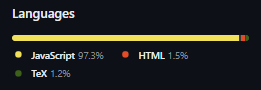
\includegraphics[width=6cm, keepaspectratio]{img/lenguajes.png}
  \caption{Porcentaje de lenguajes usados.}
  \label{fig:lenguajes}
\end{figure}


\section{Importaciones de bibliotecas JavaScript} 
\label{sec:importaciones}

\begin{itemize}
  \item \textbf{THREE.js:} Biblioteca JavaScript de código abierto para crear y renderizar gráficos en 3D en el navegador web.
  
  \item \textbf{VRButton.js:} Módulo de Three.js que facilita la integración de botones para activar la funcionalidad de realidad virtual (VR) en aplicaciones web.
  
  \item \textbf{XRControllerModelFactory.js:} Módulo de Three.js que proporciona una fábrica para crear modelos de controladores de realidad extendida (XR) para 
  su uso en aplicaciones de realidad virtual y aumentada.

  \item \textbf{Stats.js:} Módulo de Three.js que ofrece una utilidad para monitorear el rendimiento (FPS, uso de memoria) de aplicaciones web 3D en tiempo real.
  
  \item \textbf{OrbitControls.js:} Módulo de Three.js que proporciona controles de órbita para permitir al usuario rotar, acercar y alejar la cámara en una escena 3D de manera interactiva.
  
\end{itemize}


\section{Herramientas de desarrollo} 
\label{sec:herramientas}

\begin{itemize}
  \item \textbf{FireFox:} Navegador web de código abierto conocido por su enfoque en la privacidad y la personalización.
  
  \item \textbf{VisualStudioCode:} Editor de código fuente de Microsoft altamente personalizable y de código abierto, conocido 
  por su rendimiento y amplia gama de extensiones.
  
  \item \textbf{GitHub:} Plataforma de desarrollo colaborativo de software basada en la nube, que permite a los desarrolladores alojar, revisar, 
  colaborar y desplegar proyectos de software, incluidas aplicaciones web, de manera eficiente y transparente.

  \item \textbf{Oculus Quest 2:} Gafas de realidad virtual autónomas producidas por Oculus (una subsidiaria de Facebook), conocidas 
  por su alta calidad y facilidad de uso. Estas gafas fueron proporcionadas por la universidad para el desarrollo del proyecto.
  
  \item \textbf{Web XR API Emulator:} Herramienta de desarrollo que permite probar y depurar experiencias de realidad virtual y aumentada 
  basadas en WebXR directamente en el navegador web. 
  
\end{itemize}


%%%%%%%%%%%%%%%%%%%%%%%%%%%%%%%%%%%%%%%%%%%%%%%%%%%%%%%%%%%%%%%%%%%%%%%%%%%%%%%%
%%%%%%%%%%%%%%%%%%%%%%%%%%%%%%%%%%%%%%%%%%%%%%%%%%%%%%%%%%%%%%%%%%%%%%%%%%%%%%%%
% DISEÑO E IMPLEMENTACIÓN %
%%%%%%%%%%%%%%%%%%%%%%%%%%%%%%%%%%%%%%%%%%%%%%%%%%%%%%%%%%%%%%%%%%%%%%%%%%%%%%%%

\cleardoublepage
\chapter{Diseño e implementación}
\label{chap:diseno}

En este capítulo, se detalla el desarrollo del proyecto, incluyendo su estructura, los componentes en el entorno 
inmersivo, su funcionamiento, y las interacciones implementadas.


\section{Arquitectura general} 
\label{sec:arquitectura}

El proyecto se estructura en cinco componentes enlazados entre si, representados en la figura~\ref{fig:arquitectura}. Estos componentes serán explicados a continuación:

\begin{itemize}
  \item \textbf{index.html:} Representamos la estructura básica de una página web para una experiencia de realidad virtual (VR). 
  Se define un documento HTML con metadatos y referencias a archivos externos, incluyendo la biblioteca Three.js para gráficos 3D. 
  
  Además, se importa un módulo de JavaScript que inicializa la aplicación VR, creando una instancia de la clase "App" y asignándola a la ventana del navegador. 
  
  Este archivo proporciona una base para el desarrollo de aplicaciones de realidad virtual en la web.
  
  \item \textbf{app.js:} Este script es una aplicación que utiliza la biblioteca Three.js para crear una escena 3D interactiva. Que realiza:
    
    \begin{enumerate}
      \item Importa las bibliotecas necesarias de Three.js para crear la escena.
      \item Carga varias texturas de imágenes para aplicarlas a los materiales de los objetos en la escena.
      \item Define algunas variables y objetos necesarios para el funcionamiento de la aplicación.
      \item Crea una clase App que inicializa la escena, la cámara, la iluminación y los controles.
      \item Dentro de la clase App, hay métodos para manejar el control de los dispositivos de entrada de VR, como los controladores y sus eventos.
      \item Contiene un método para construir los modelos de los controladores de VR.
      \item Otro método se encarga de manejar la lógica de la animación y la interacción del usuario con la escena.
      \item Y finalmente, tenemos un método de renderizado que se ejecuta en bucle y actualiza la escena en cada fotograma.
    \end{enumerate}

  \item \textbf{imágenes:} En la arquitectura del proyecto, tenemos una carpeta llamada "imagenes" que contiene todas las imágenes utilizadas en la aplicación. 
  Dentro de esta carpeta, tenemos subcarpetas para organizar las imágenes de acuerdo con su propósito.

  Cada imagen se carga en la aplicación utilizando el constructor THREE.TextureLoader().load(), 
  proporcionando la ruta relativa desde el punto donde se está ejecutando el código hacia la ubicación de la imagen en la estructura de carpetas.

  \item \textbf{sceneObjets:} Este archivo es un módulo de funciones que proporciona diferentes objetos tridimensionales (3D) utilizando la biblioteca Three.js. 
  Cada función devuelve un objeto con geometría y material específicos.

  \begin{enumerate}
    \item \textbf{Sphere:} Devuelve una esfera roja con una geometría esférica y un material básico.
    \item \textbf{Side:} Devuelve un objeto rectangular con una textura proporcionada, usado como pared en la escena.
    \item \textbf{Box:} Devuelve una caja con una textura proporcionada, usado como UA y Proxy en la escena.
    \item \textbf{Wall:} Devuelve un plano grande con una textura proporcionada, usado como pantalla en la escena.
    \item \textbf{Logo:} Devuelve un plano con una textura proporcionada, representando logotipo.
    \item \textbf{Floor:} Devuelve un plano grande con una textura proporcionada, usado para el suelo de la escena.
  \end{enumerate}

  Cada función utiliza diferentes geometrías y materiales para crear los objetos 3D. 
  También configura propiedades específicas de los materiales, como envoltura de textura y repetición.
  
  \item \textbf{jsm:} Esta carpeta contiene módulos JavaScript utilizados en el proyecto. Estos módulos son archivos independientes que proporcionan funcionalidades específicas para la aplicación. 
  Aquí está la estructura de la carpeta:

  \begin{enumerate}
    \item \textbf{build:} En esta subcarpeta se encuentran los archivos de construcción de la biblioteca Three.js, 
    que proporcionan la funcionalidad principal de renderización en 3D. El archivo principal utilizado es three.module.js, 
    que importa todas las funcionalidades esenciales de Three.js.
    \item \textbf{webxr:} Aquí están los módulos relacionados con WebXR, una API que permite crear experiencias de realidad virtual (VR) y realidad aumentada (AR) en el navegador. 
    Por ejemplo, VRButton.js proporciona un botón para activar la experiencia de realidad virtual, mientras que XRControllerModelFactory.js 
    permite crear modelos visuales para los controladores de VR.
    \item \textbf{libs:} Esta subcarpeta contiene bibliotecas adicionales utilizadas en el proyecto. 
    En particular, stats.module.js proporciona una herramienta para medir el rendimiento de la aplicación 
    mediante la visualización de estadísticas, como el número de fotogramas por segundo.
    \item \textbf{controls:} Aquí están los módulos relacionados con el control de la cámara y la escena en la aplicación. 
    Por ejemplo, OrbitControls.js proporciona controles para permitir al usuario mover y rotar la cámara 
    alrededor de la escena, lo que facilita la navegación en entornos 3D.
  \end{enumerate}

  Por lo tanto, la carpeta 'jsm' organiza los módulos JavaScript utilizados en el proyecto, 
  proporcionando funcionalidades esenciales, soporte para WebXR, herramientas de medición de rendimiento y controles de cámara. 
  Estos módulos se importan en la aplicación según sea necesario para agregar las características deseadas.

\end{itemize}

\begin{figure}
  \centering
  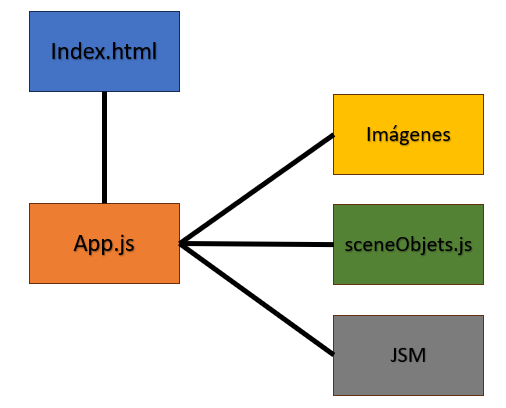
\includegraphics[width=9cm, keepaspectratio]{img/estructura.png}
  \caption{Estructura del proyecto}
  \label{fig:arquitectura}
\end{figure}


\section{Escena} 
\label{sec:escena}

La escena virtual implementada se desarrolla utilizando la biblioteca Three.js, 
que permite la creación de gráficos 3D en un entorno web. Este proyecto configura un entorno interactivo 
que simula un sistema de comunicación, donde se pueden visualizar los intercambios de mensajes entre diferentes usuarios y un proxy.

\textbf{Estructura básica}

\begin{itemize}
  \item \textbf{Cámara y Controles:} La cámara se configura con una perspectiva que permite al usuario tener una vista adecuada del entorno virtual. 
  Se utiliza OrbitControls para permitir al usuario interactuar con la vista, rotando y acercando/alejando la escena.
  
  \item \textbf{Iluminación:} Se añade iluminación hemisférica para simular una luz suave y direccional 
  para destacar objetos específicos dentro de la escena.

  \item \textbf{Renderizado:} Se establece un renderizado con antialiasing para mejorar la calidad visual de los bordes de los objetos en la escena.
  
\end{itemize}

\textbf{Objetos en la escena}

\begin{itemize}
  \item \textbf{Suelo y paredes:} Se utilizan texturas cargadas para crear un suelo y paredes que encierran la escena, proporcionando un fondo estático.
  
  \item \textbf{Objetos interactivos:} Se crean varias cajas y esferas que representan a diferentes usuarios (UA1, UA2) y un proxy. 
  Estos objetos se pueden interactuar mediante eventos controlados por los controladores de realidad virtual.

  \item \textbf{Indicadores visuales:} Se utilizan logos y texturas para indicar estados como "start" y "stop", mostrando visualmente el flujo de la simulación.
  
\end{itemize}

\textbf{Interacción y dinámica}

\begin{itemize}
  \item \textbf{Inicio de eventos:} La interacción comienza cuando el usuario activa controles específicos en los controladores de realidad virtual. 
  Esto puede alterar el estado de los objetos (por ejemplo, cambiar el color para indicar actividad) y cambiar texturas que 
  representan diferentes mensajes enviados y recibidos en la comunicación.
  
  \item \textbf{Simulación de mensajes:} Los objetos esféricos se mueven entre las cajas para simular el envío de mensajes. 
  La ruta y la dirección de estos objetos dependen de las interacciones del usuario y el flujo del protocolo simulado.

  \item \textbf{Animación de paquetes RTP:} En ciertos puntos, esferas adicionales se mueven para simular la transmisión de paquetes RTP, 
  indicando el intercambio de media en una llamada establecida.
  
\end{itemize}


\textbf{Implementación}

\begin{itemize}
  \item \textbf{Controladores XR:} Se configuran controladores para manejar la interacción en un entorno de realidad extendida (XR). 
  Esto incluye la gestión de eventos de selección y conexión de dispositivos.
  
  \item \textbf{Animación y actualización de la escena:} Los objetos esféricos se mueven entre las cajas para simular el envío de mensajes. 
  La ruta y la dirección de estos objetos dependen de las interacciones del usuario y el flujo del protocolo simulado.

  \item \textbf{Animación de paquetes RTP:} La lógica para mover objetos y actualizar estados se ejecuta dentro de un bucle 
  de animación que recalcula posiciones y estados basados en la interacción del usuario.
  
\end{itemize}

\begin{figure}
  \centering
  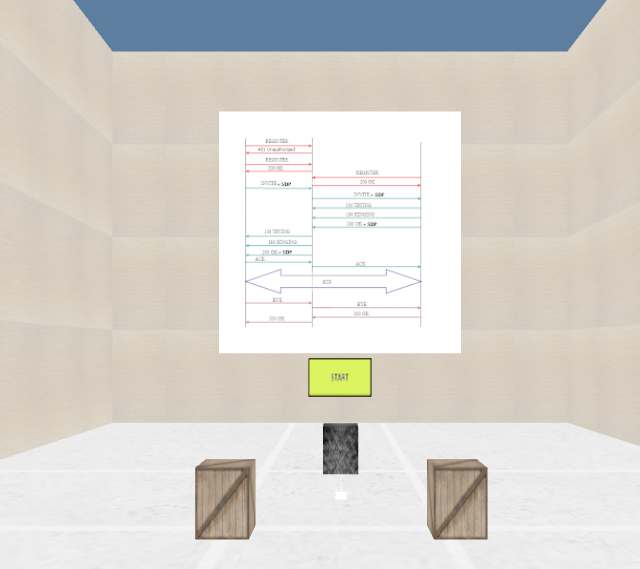
\includegraphics[width=9cm, keepaspectratio]{img/escena.png}
  \caption{Escena del proyecto}
  \label{fig:arquitectura}
\end{figure}


\section{Controles de realidad virtual}
\label{sec:controles_vr}

La implementación de controles de realidad virtual en la aplicación proporciona una interfaz interactiva que mejora significativamente la experiencia del usuario, 
permitiendo una manipulación intuitiva y directa de la escena virtual.

\subsection{Configuración de los controladores VR}
\label{subsec:configuracion_controladores_vr}

Los controladores VR son dispositivos físicos que los usuarios sostienen en sus manos y que detectan sus movimientos y gestos en el espacio tridimensional. 
Estos están equipados con una variedad de sensores y botones que permiten una gama amplia de interacciones:

\begin{itemize}
  \item \textbf{Botones y Gatillos}: Utilizados para realizar selecciones y activar eventos dentro de la aplicación. 
  Por ejemplo, un usuario puede iniciar la transmisión de mensajes al presionar el botón "Start".
  \item \textbf{Sensores de Movimiento}: Capturan el posicionamiento y la orientación de las manos del usuario, 
  permitiendo manipular objetos o navegar por la escena con movimientos naturales.
\end{itemize}

\begin{figure}
  \centering
  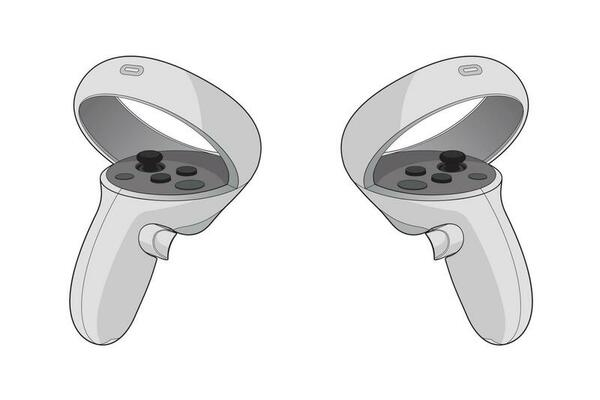
\includegraphics[width=6cm, keepaspectratio]{img/controlador.png}
  \caption{Controlador VR}
  \label{fig:controlador}
\end{figure}


\subsection{Interacción mediante controladores VR}
\label{subsec:interaccion_controladores_vr}

La interacción con la escena se realiza a través de los controladores VR de la siguiente manera:

\begin{itemize}
  \item \textbf{Selección y Manipulación}: Los usuarios apuntan a objetos virtuales con los controladores y utilizan 
  botones para seleccionarlos. Esto puede incluye activar elementos dentro de la escena.
  \item \textbf{Navegación}: Mediante el uso del gatillo en los controladores, 
  los usuarios pueden desplazarse por la escena virtual, acercándose o alejándose de los objetos o desplazándose lateralmente.
  \item \textbf{Interacción Contextual}: La aplicación cambia la funcionalidad de la escena 
  basándose el estado del objeto con el que el usuario está interactuando, 
  cambiando modos de visualización o ajustando parámetros específicos de los objetos.
\end{itemize}

\subsection{Implementación técnica}
\label{subsec:implementacion_tecnica_vr}

La implementación técnica de los controladores VR en la aplicación utiliza la API de WebXR, integrada con Three.js, para gestionar la entrada 
de los dispositivos de realidad virtual. El código configura cada controlador para responder a eventos como `selectstart` y `selectend`, 
lo que permite detectar interacciones como pulsaciones de botones y liberaciones. Adicionalmente, se emplean rayos virtuales (`raycasting`) 
para determinar qué objetos están siendo apuntados por los controladores, facilitando así una interacción precisa.


En la implementación de la aplicación, hacemos un uso específico de los botones trigger de los controladores VR para facilitar una interacción 
intuitiva y efectiva dentro del entorno virtual. Cada trigger tiene un propósito bien definido que mejora la experiencia del 
usuario y la funcionalidad de la aplicación:

\begin{itemize}
  \item \textbf{Trigger del controlador izquierdo}: Este botón se utiliza para la navegación dentro de la escena. Al presionar el trigger del controlador izquierdo, 
  el usuario puede desplazarse hacia donde esté mirando con las gafas de realidad virtual, lo que permite una navegación intuitiva y natural. 
  Esta funcionalidad es fundamental para explorar diferentes áreas de la escena de manera fluida.
  
  \item \textbf{Trigger del controlador derecho}: El trigger del controlador derecho está configurado para interactuar con objetos 
  específicos de la escena. Cuando se presiona este botón, se puede seleccionar o activar elementos dentro de la escena, 
  como iniciar una simulación, modificar parámetros de un objeto, o ejecutar acciones específicas relacionadas con los objetos con los que se interactúa. 
  Esta interacción es esencial para manipular elementos de la aplicación y para participar activamente en las simulaciones y demostraciones que se presentan en el entorno virtual.
\end{itemize}

La programación de estos triggers se realiza a través del manejo de eventos en JavaScript, utilizando la API de WebXR para detectar y responder 
a las acciones del usuario. Este diseño permite un control preciso sobre la aplicación, ofreciendo a los usuarios una manera clara y directa 
de interactuar con la interfaz y con los elementos virtuales de la escena.

\begin{figure}
  \centering
  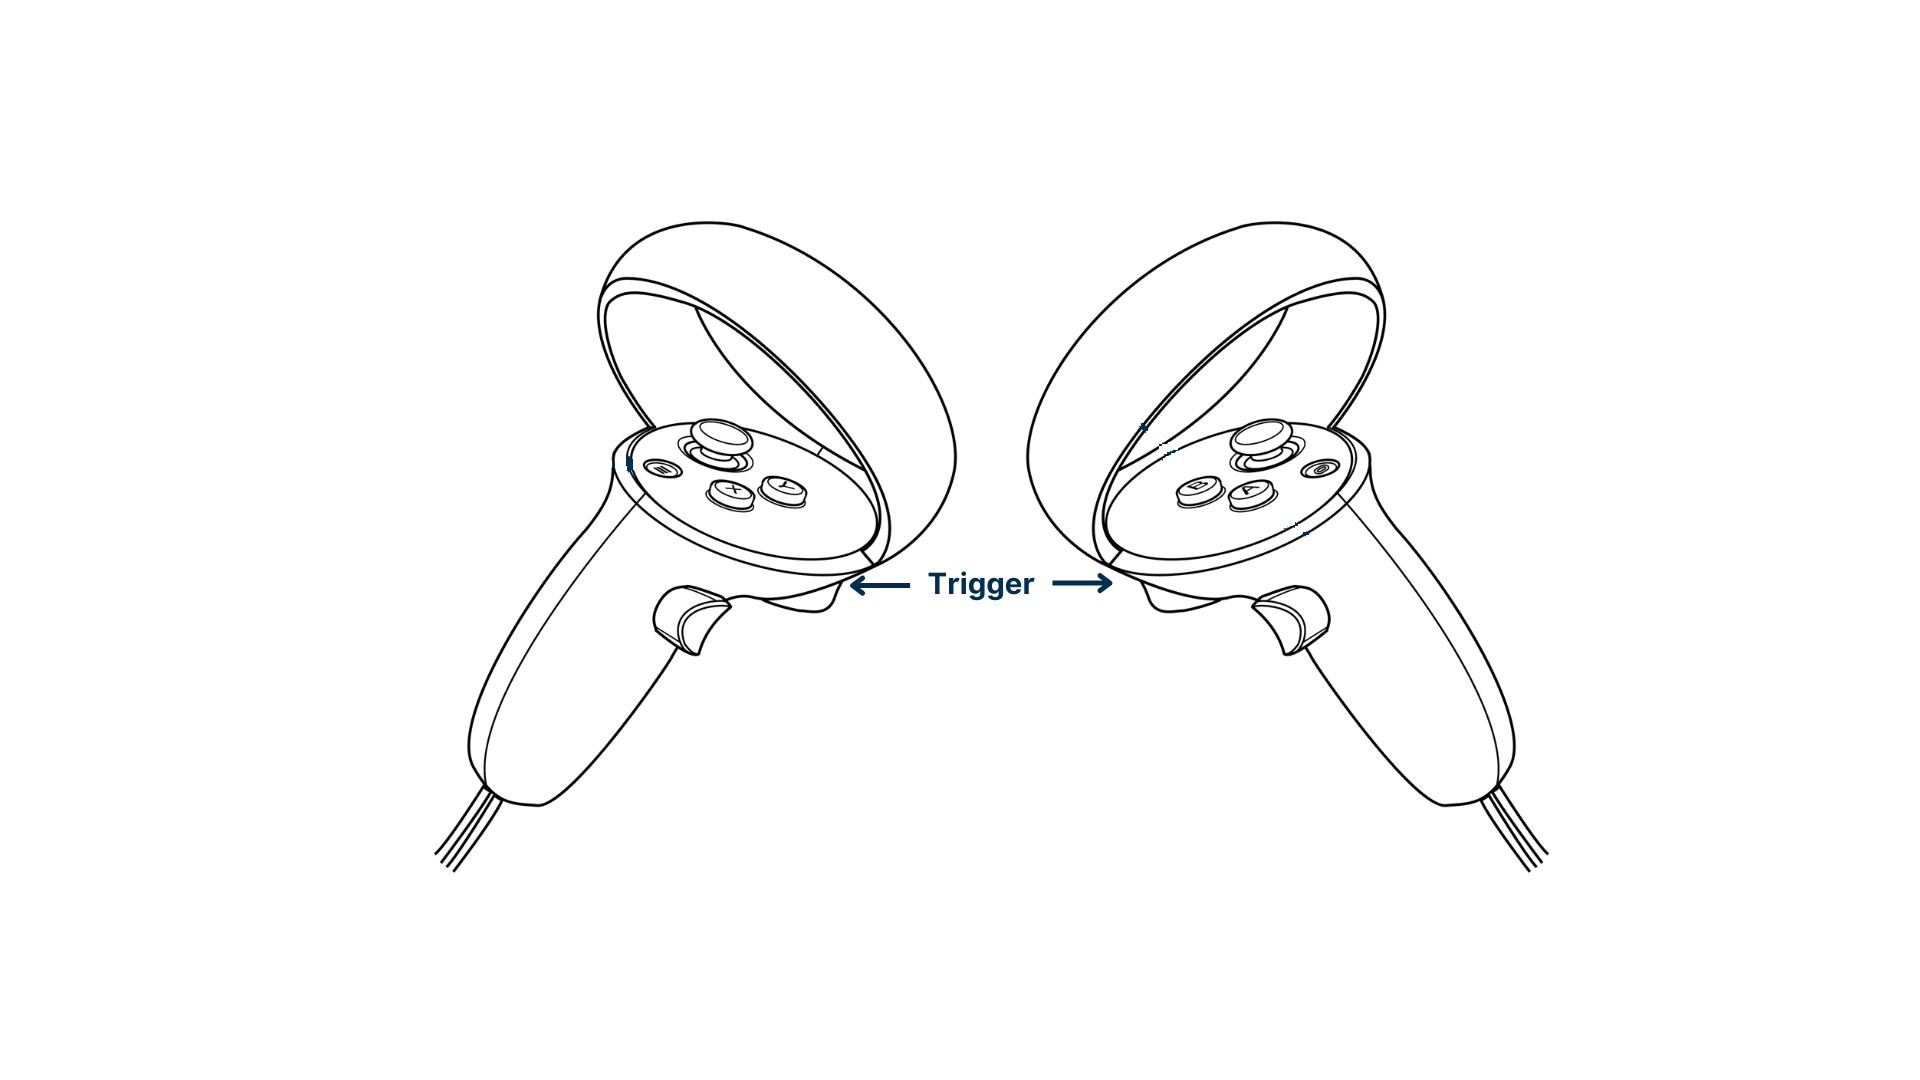
\includegraphics[width=6cm, keepaspectratio]{img/BotonesControlador.png}
  \caption{Botones controlador VR}
  \label{fig:controladorBotones}
\end{figure}


%%%%%%%%%%%%%%%%%%%%%%%%%%%%%%%%%%%%%%%%%%%%%%%%%%%%%%%%%%%%%%%%%%%%%%%%%%%%%%%%
%%%%%%%%%%%%%%%%%%%%%%%%%%%%%%%%%%%%%%%%%%%%%%%%%%%%%%%%%%%%%%%%%%%%%%%%%%%%%%%%
% RESULTADOS %
%%%%%%%%%%%%%%%%%%%%%%%%%%%%%%%%%%%%%%%%%%%%%%%%%%%%%%%%%%%%%%%%%%%%%%%%%%%%%%%%

\cleardoublepage
\chapter{Resultados}
\label{chap:resultados}

En este capítulo, se presentan los resultados derivados de las interacciones con los objetos de la escena en la aplicación 
de realidad virtual desarrollada. Se describirá cómo distintas selecciones de objetos generan resultados visuales y 
funcionales diferentes, lo que demuestra la dinámica y la reactividad de la aplicación ante las acciones del usuario.

\section{Descripción de las interacciones}
\label{sec:descripcion_interacciones}
Las interacciones en la aplicación permiten a los usuarios seleccionar objetos virtuales, 
los cuales alteran el estado de la escena y desencadenan eventos específicos. 

Como se mencionó en la Sección 4.3.3, para lograr estos resultados es necesario utilizar controladores VR. 
Estos dispositivos permiten a los usuarios moverse por la escena e interactuar con los objetos de manera intuitiva y efectiva.
La selección se realiza apuntando hacia el objeto con el controlador derecho y activando el trigger.

Cada objeto tiene asociadas consecuencias específicas que se detallan a continuación:

\subsection{Interacción con UA1}
\label{subsec:objeto_ua1}

Este objeto representa un usuario dentro del entorno virtual y está visualizado como una caja 
de madera ubicada en la parte izquierda de la escena.

Al interactuar con UA1, este cambiará de color y podrán obtener dos posibles resultados, los cuales dependen 
de si el intercambio de paquetes ha sido inicializado o no.

\subsubsection{Intercambio de paquetes no iniciado}
\label{subsubsec:Intercambio_NoIniciado}
Si el intercambio de paquetes no ha sido inicializado, en la pantalla situada en la pared central se mostrarán 
los atributos del usuario en estado vacío, indicando los valores que deberían ser completados, mostrados en la figura~\ref{fig:UA1_NoIniciado}. 
Esta visualización es esencial para comprender los requisitos iniciales de configuración del usuario en la red. Estos tributos son:

\begin{itemize}
  \item \textbf{'account'}: ['username', 'passwd']
  \item \textbf{'uaserver'}: ['ip', 'puerto']
  \item \textbf{'rtpaudio'}: ['puerto']
  \item \textbf{'regproxy'}: ['ip', 'puerto']
  \item \textbf{'log'}: ['path']
  \item \textbf{'audio'}: ['path']
\end{itemize}

\begin{figure}
  \centering
  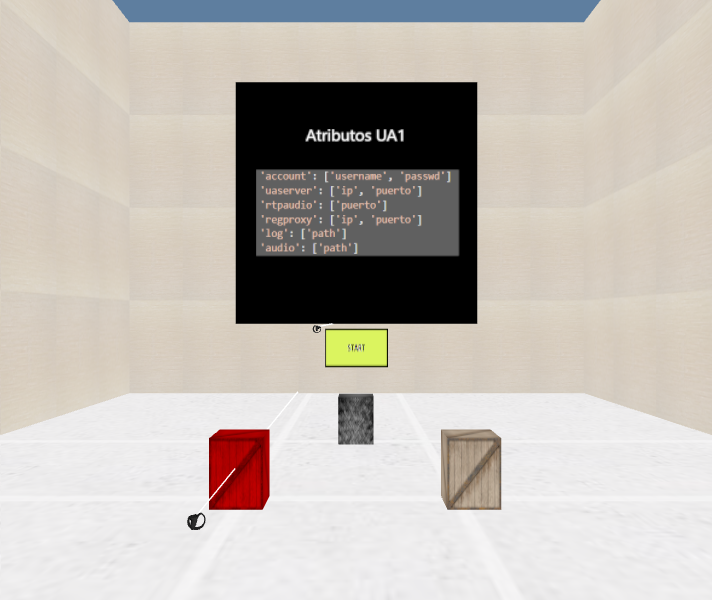
\includegraphics[width=15cm, keepaspectratio]{img/resultados/UA1_NoIniciado.png}
  \caption{Estado inicial del UA1}
  \label{fig:UA1_NoIniciado}
\end{figure}


\subsubsection{Intercambio de paquetes iniciado}
\label{subsubsec:Intercambio_Iniciado}
Una vez que el intercambio de paquetes ha sido iniciado, en la misma pantalla se 
actualizarán los atributos del usuario con valores específicos y correctos para su funcionamiento mostrados en la figura~\ref{fig:UA1_Iniciado}.  
Este cambio refleja cómo el sistema procesa y responde a las interacciones, ofreciendo un feedback visual del estado operativo del usuario.

\begin{figure}
  \centering
  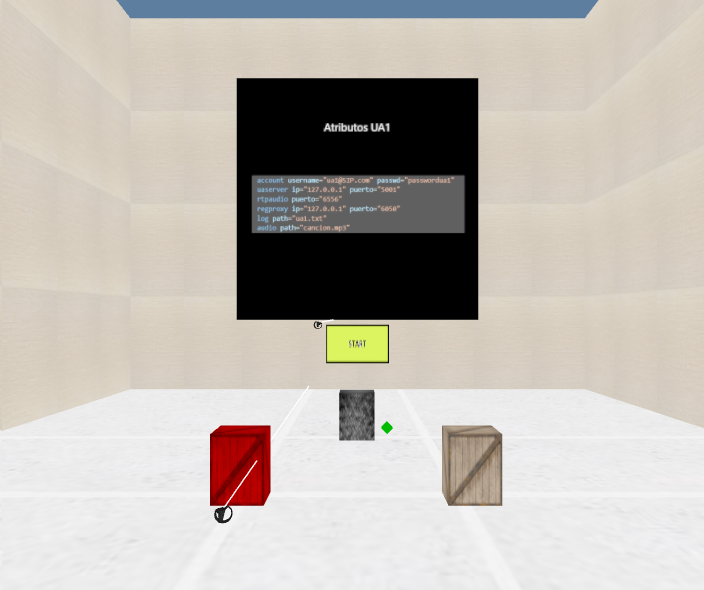
\includegraphics[width=15cm, keepaspectratio]{img/resultados/UA1_Iniciado.png}
  \caption{Atributos UA1 con valores específicos}
  \label{fig:UA1_Iniciado}
\end{figure}


\subsection{Interacción con el proxy}
\label{subsec:objeto_proxy}

Este objeto representa un servidor proxy en el entorno virtual y está visualizado como una caja con textura oscura,
ubicada en la parte central de la escena.

Al interactuar con el Proxy, este cambiará de color y dependiendo del estado de la interacción con los usuarios (UA1 y UA2), 
se pueden obtener diferentes resultados, influenciados por si el intercambio de paquetes ha sido iniciado o no.

\subsubsection{Intercambio de paquetes no iniciado}
\label{subsubsec:Proxy_Intercambio_NoIniciado}
Si el intercambio de paquetes no ha sido inicializado, la interacción con el Proxy mostrará en la pantalla sus atributos 
con la información que deben ser completados, donde no se procesan aún los paquetes, mostrados en la figura~\ref{fig:Proxy_NoIniciado}. Estos campos son:

\begin{itemize}
  \item \textbf{'server'}: ['name', 'ip', 'puerto']
  \item \textbf{'database'}: ['path', 'passwdpath']
  \item \textbf{'log'}: ['path']
\end{itemize}

\begin{figure}
  \centering
  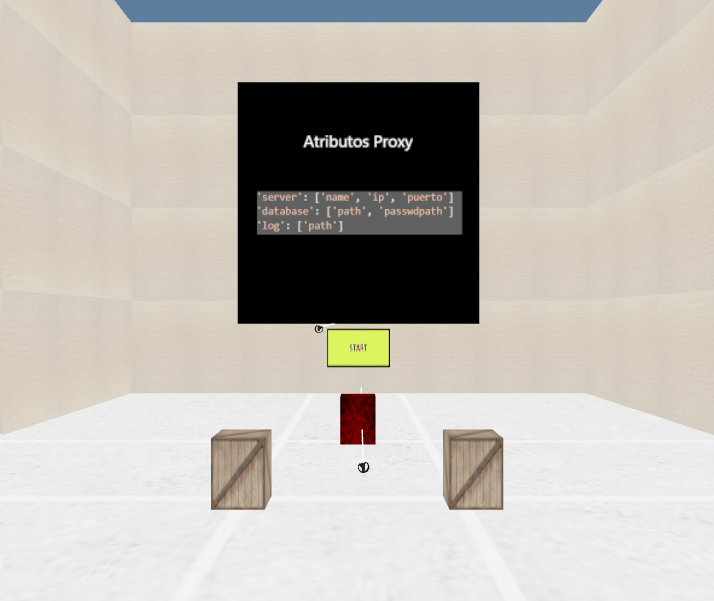
\includegraphics[width=15cm, keepaspectratio]{img/resultados/Proxy_NoIniciado.png}
  \caption{Estado inicial del Proxy}
  \label{fig:Proxy_NoIniciado}
\end{figure}

\subsubsection{Intercambio de paquetes iniciado}
\label{subsubsec:Proxy_Intercambio_Iniciado}
Una vez que el intercambio de paquetes ha sido iniciado, el Proxy procesará y dirigirá los paquetes entre los usuarios correspondientes, 
reflejando este flujo en la interfaz con actualizaciones dinámicas. Al seleccionar el Proxy se mostrarán sus atributos con valores específicos 
y correctos para su funcionamiento, mostrados en la figura~\ref{fig:Proxy_Iniciado}.

\begin{figure}
  \centering
  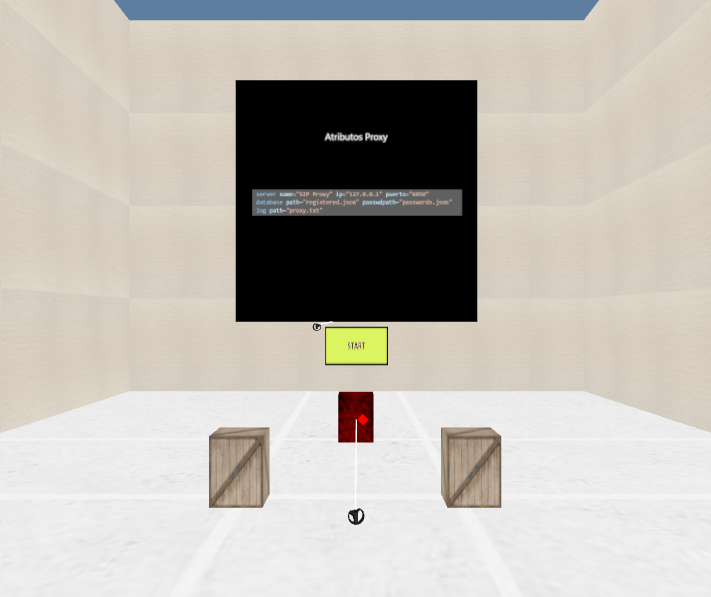
\includegraphics[width=15cm, keepaspectratio]{img/resultados/Proxy_Iniciado.png}
  \caption{Atributos Proxy con valores específicos}
  \label{fig:Proxy_Iniciado}
\end{figure}


\subsection{Interacción con UA2}
\label{subsec:objeto_ua1}

Este objeto representa un usuario dentro del entorno virtual y está visualizado como una caja 
de madera ubicada en la parte derecha de la escena.

Al interactuar con UA2, este cambiará de color y podrán obtener dos posibles resultados, los cuales dependen 
de si el intercambio de paquetes ha sido inicializado o no.

\subsubsection{Intercambio de paquetes no iniciado}
\label{subsubsec:Intercambio_NoIniciado}
Si el intercambio de paquetes no ha sido inicializado, en la pantalla situada en la pared central se mostrarán 
los atributos del usuario en estado vacío, indicando los valores que deberían ser completados, mostrados en la figura~\ref{fig:UA2_NoIniciado}. 
Esta visualización es esencial para comprender los requisitos iniciales de configuración del usuario en la red. Estos tributos son:

\begin{itemize}
  \item \textbf{'account'}: ['username', 'passwd']
  \item \textbf{'uaserver'}: ['ip', 'puerto']
  \item \textbf{'rtpaudio'}: ['puerto']
  \item \textbf{'regproxy'}: ['ip', 'puerto']
  \item \textbf{'log'}: ['path']
  \item \textbf{'audio'}: ['path']
\end{itemize}

\begin{figure}
  \centering
  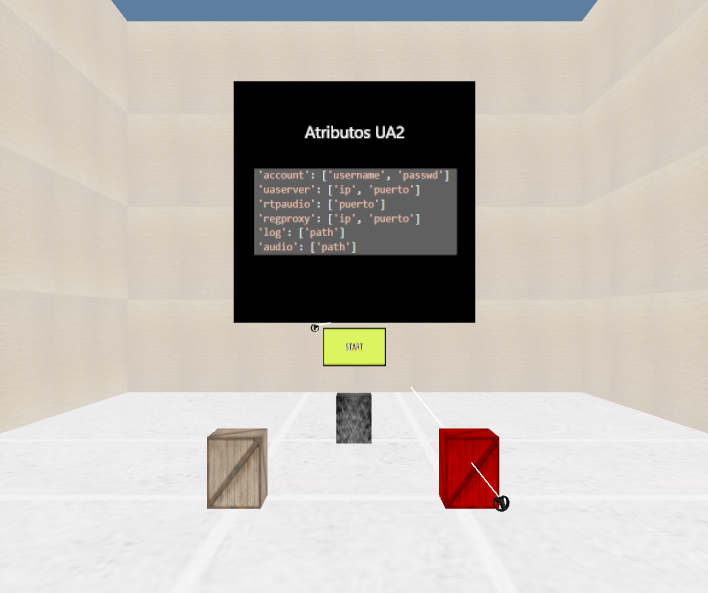
\includegraphics[width=15cm, keepaspectratio]{img/resultados/UA2_NoIniciado.png}
  \caption{Estado inicial del UA2}
  \label{fig:UA2_NoIniciado}
\end{figure}


\subsubsection{Intercambio de paquetes iniciado}
\label{subsubsec:Intercambio_Iniciado}
Una vez que el intercambio de paquetes ha sido iniciado, en la misma pantalla se 
actualizarán los atributos del usuario con valores específicos y correctos para su funcionamiento mostrados en la figura~\ref{fig:UA2_Iniciado}.  
Este cambio refleja cómo el sistema procesa y responde a las interacciones, ofreciendo un feedback visual del estado operativo del usuario.

\begin{figure}
  \centering
  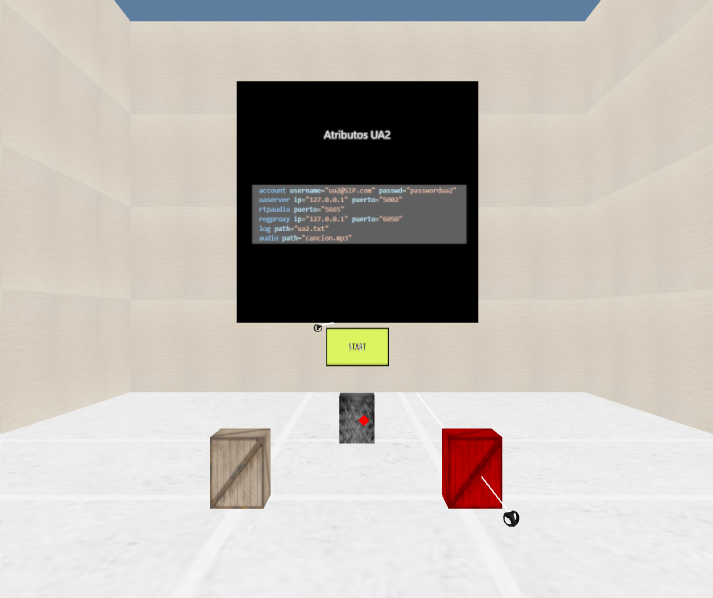
\includegraphics[width=15cm, keepaspectratio]{img/resultados/UA2_Iniciado.png}
  \caption{Atributos UA2 con valores específicos}
  \label{fig:UA2_Iniciado}
\end{figure}


\subsection{Interacción con paquetes}
\label{subsec:objeto_paquetes}
En el entorno de realidad virtual, los paquetes se representan en forma de esferas que simulan la transmisión de datos en una red. 
Estas esferas visualizan claramente el flujo de información, con un origen, un destino y un color claramente definidos, 
dependiendo del tipo de intercambio en el que participan.

Al seleccionar uno de estos paquetes, el sistema mostrará información detallada contenida en el paquete, 
incluyendo una representación visual del flujo de transmisión que indica su origen, destino y la dirección del flujo.

El proceso y secuencia de intercambio de paquetes en este proyecto se ilustra en la siguiente figura~\ref{fig:Secuencia_Paquetes}, donde se puede observar el orden 
específico seguido durante las simulaciones.

Esta figura~\ref{fig:Secuencia_Paquetes} ilustra un intercambio de mensajes de protocolo típico en una comunicación de red utilizando el Protocolo de Inicio de Sesión (SIP). 
Este diagrama de flujo representa la secuencia de mensajes entre dos usuarios que intentan establecer una comunicación, 
pasando por un proceso de registro y luego de llamada.

\begin{figure}
  \centering
  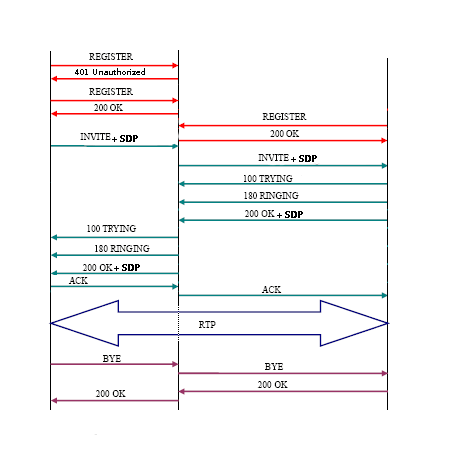
\includegraphics[width=15cm, keepaspectratio]{img/resultados/Secuencia_Paquetes.png}
  \caption{Secuencia del intercambio de paquetes}
  \label{fig:Secuencia_Paquetes}
\end{figure}

\subsubsection{Desglose de la secuencia de comunicación}
\label{subsubsec:secuencia_comunicación}

Inicialmente, el proceso comienza con un intento de registro, donde el usuario A (UA1) envía un mensaje REGISTER al servidor, 
representado en la figura~\ref{fig:01-Register_UA1}. 
Si no está autorizado, recibe un 401 Unauthorized, mostrado en la figura~\ref{fig:02-Unautorized}, 
lo que obliga al usuario (UA1) a realizar otro intento de REGISTER, el cual, es aceptado,
y se confirma con una respuesta 200 OK, ilustrado en la figura~\ref{fig:02-200OK}, 
indicando que el registro se ha completado con éxito.
\bigskip

A continuación, se registra el usuario B (UA2) enviando un mensaje REGISTER al servidor,
representado en la figura~\ref{fig:03-Register_UA2}. 
Siendo este aceptado y confirmado con una respuesta de 200 OK, ilustrado en la figura~\ref{fig:04-200OK}.
\bigskip

La fase de llamada comienza con un INVITE acompañado de una descripción de la sesión (SDP), escenificado en la figura~\ref{fig:05-Invite}, 
que contiene los detalles para establecer la comunicación. 
Este mensaje es respondido con un 100 TRYING, evidenciado en la figura~\ref{fig:07-Trying},
seguido de un 180 RINGING, ilustrado en la figura~\ref{fig:08-Ringing}, 
que indica que la llamada está siendo procesada y que el otro usuario está siendo alertado de la llamada entrante. 
Cuando el usuario B (UA2) acepta la llamada, envía una respuesta 200 OK + SDP, representado en la figura~\ref{fig:09-200OKSDP}, 
que contiene la confirmación y los detalles necesarios para establecer la comunicación. 
El usuario A (UA1) confirma recibir esta información con un ACK, mostrado en la figura~\ref{fig:13-ACK}.
\bigskip

Una vez establecida la llamada, los datos multimedia se transmiten a través de 
paquetes RTP (Protocolo de Transporte en Tiempo Real), escenificado en la figura~\ref{fig:15-RTP}, 
representados por las esferas azules. Este intercambio continúa hasta que uno de los usuarios decide terminar la llamada, 
enviando un mensaje BYE, ilustrado en la figura~\ref{fig:16-BYE}. 
El fin de la llamada es confirmado por el otro usuario con un 200 OK, representado en la figura~\ref{fig:18-200OK}, 
cerrando así la sesión de comunicación.
% Bloque 1 %
\begin{figure}
  \centering
  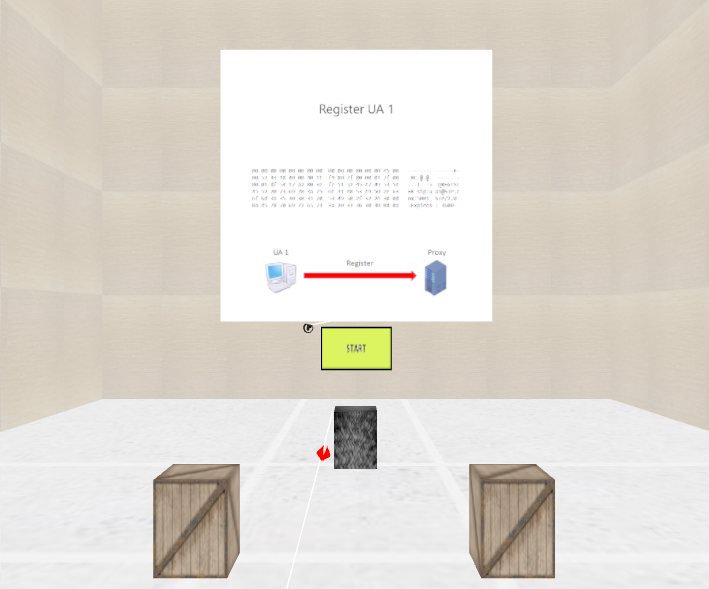
\includegraphics[width=12cm, keepaspectratio]{img/resultados/01-Register_UA1.png}
  \caption{Mensaje de registro inicial de UA1}
  \label{fig:01-Register_UA1}
\end{figure}

\begin{figure}
  \centering
  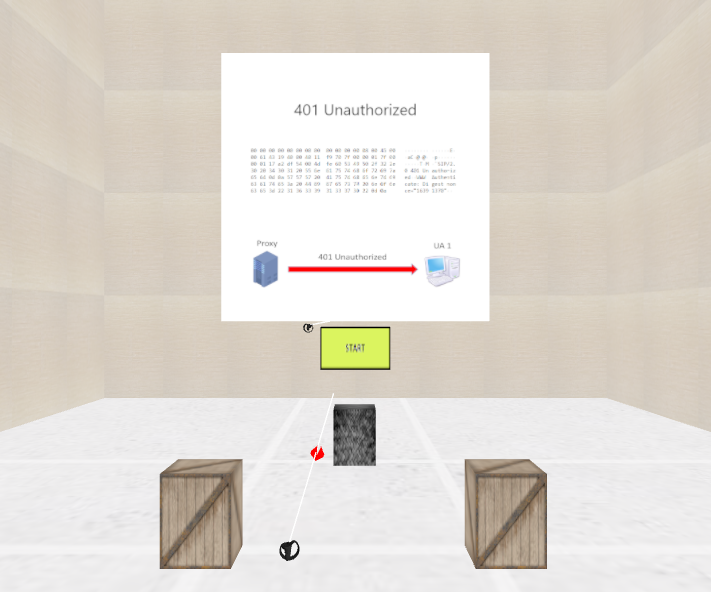
\includegraphics[width=12cm, keepaspectratio]{img/resultados/02-Unautorized.png}
  \caption{Respuesta 401 Unauthorized a UA1}
  \label{fig:02-Unautorized}
\end{figure}

\begin{figure}
  \centering
  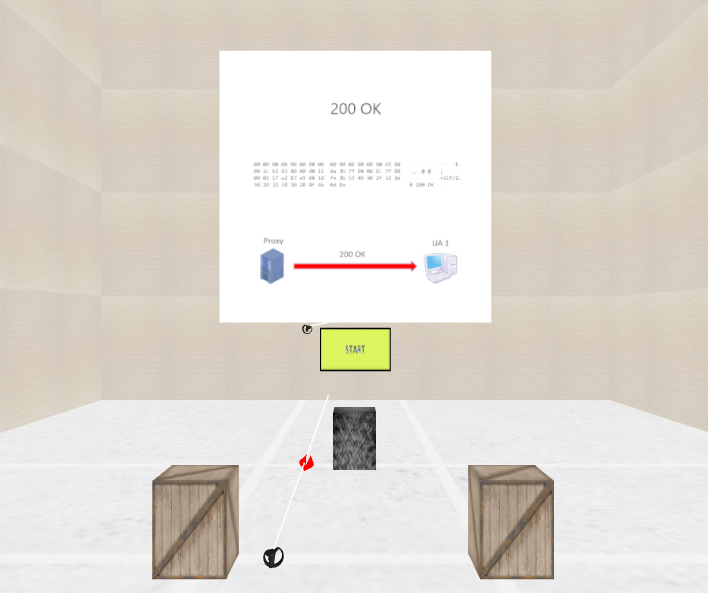
\includegraphics[width=12cm, keepaspectratio]{img/resultados/02-200OK.png}
  \caption{Registro de UA1 exitoso con 200 OK}
  \label{fig:02-200OK}
\end{figure}
% Bloque 2 %
\begin{figure}
  \centering
  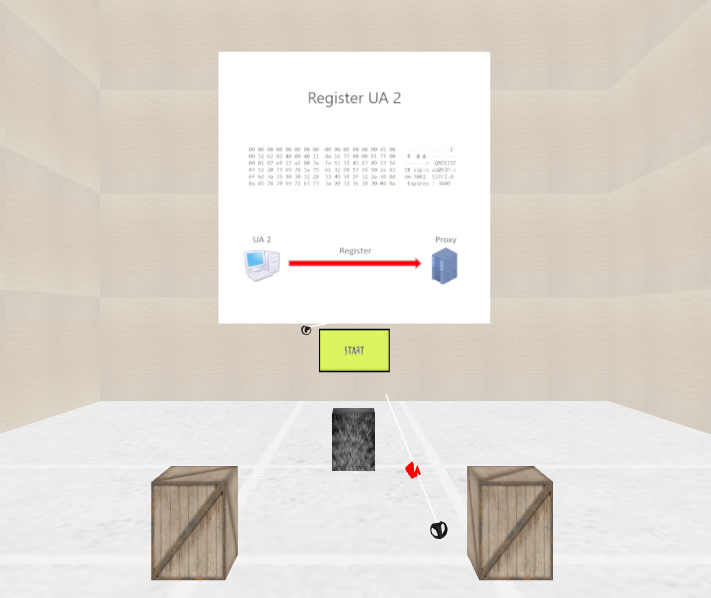
\includegraphics[width=12cm, keepaspectratio]{img/resultados/03-Register_UA2.png}
  \caption{Mensaje de registro inicial de UA2}
  \label{fig:03-Register_UA2}
\end{figure}

\begin{figure}
  \centering
  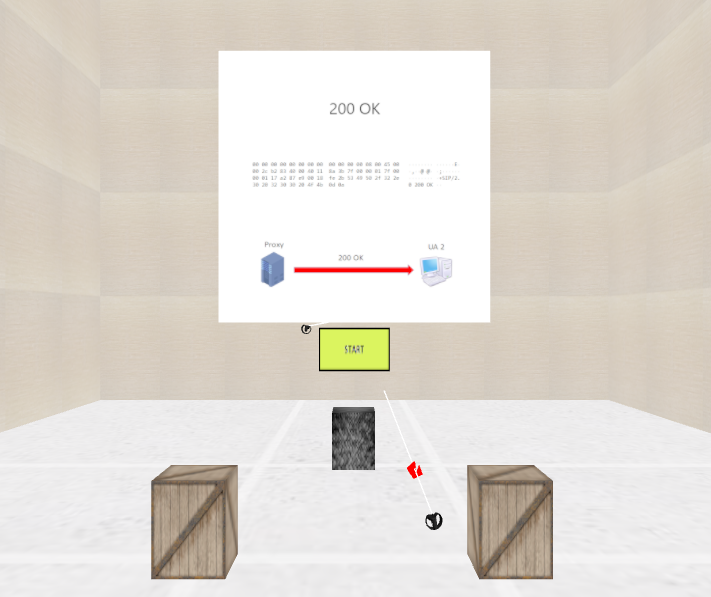
\includegraphics[width=12cm, keepaspectratio]{img/resultados/04-200OK.png}
  \caption{Registro de UA2 exitoso con 200 OK}
  \label{fig:04-200OK}
\end{figure}

% Bloque 3 %
\begin{figure}
  \centering
  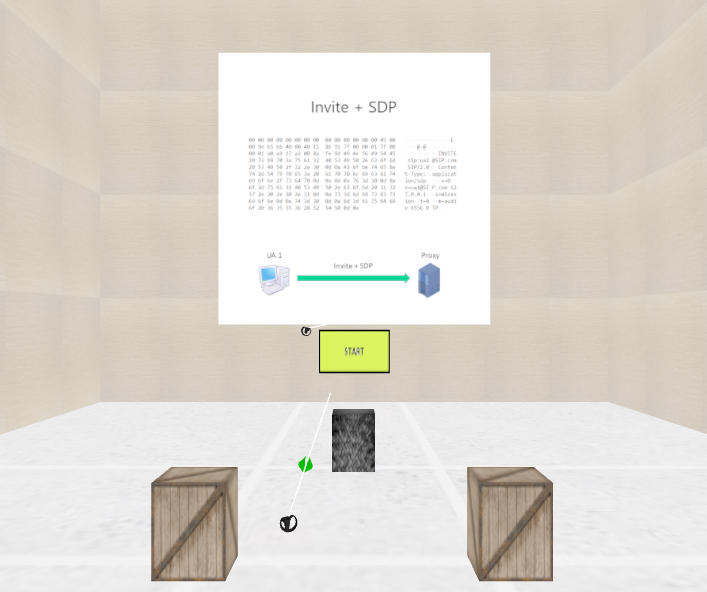
\includegraphics[width=12cm, keepaspectratio]{img/resultados/05-Invite.png}
  \caption{Inicio de llamada con el mensaje INVITE de UA1}
  \label{fig:05-Invite}
\end{figure}

\begin{figure}
  \centering
  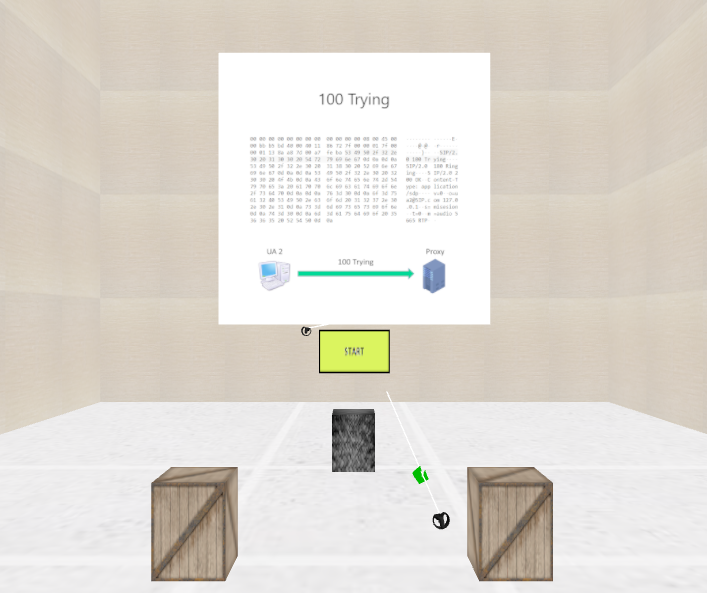
\includegraphics[width=12cm, keepaspectratio]{img/resultados/07-Trying.png}
  \caption{Respuesta TRYING de UA2 indicando procesamiento}
  \label{fig:07-Trying}
\end{figure}

\begin{figure}
  \centering
  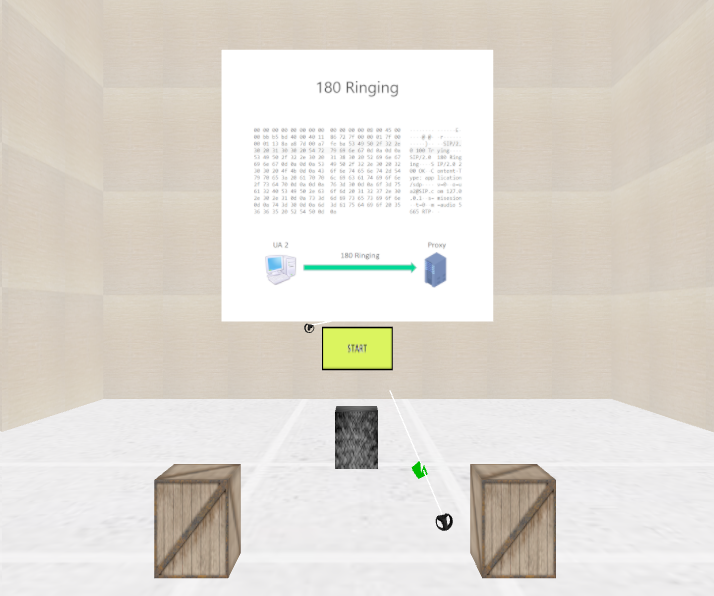
\includegraphics[width=12cm, keepaspectratio]{img/resultados/08-Ringing.png}
  \caption{Alerta de llamada con el mensaje RINGING de UA2}
  \label{fig:08-Ringing}
\end{figure}

\begin{figure}
  \centering
  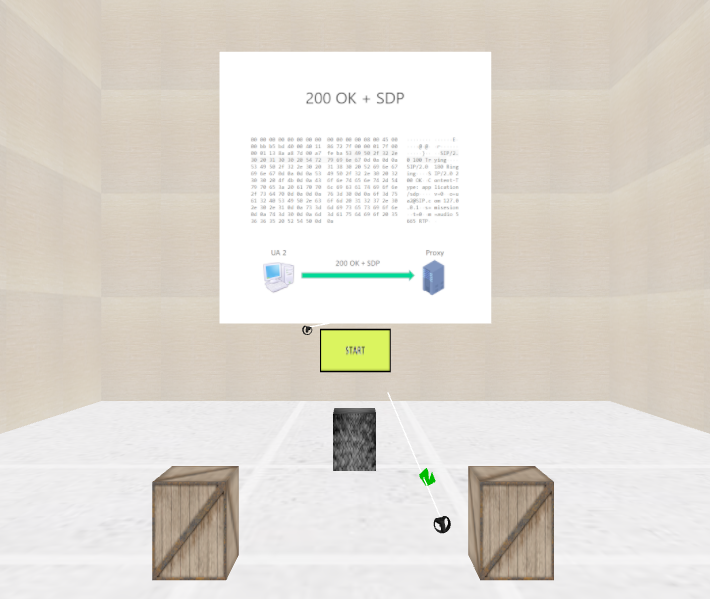
\includegraphics[width=12cm, keepaspectratio]{img/resultados/09-200OKSDP.png}
  \caption{Confirmación de llamada con 200 OK + SDP de UA2}
  \label{fig:09-200OKSDP}
\end{figure}

\begin{figure}
  \centering
  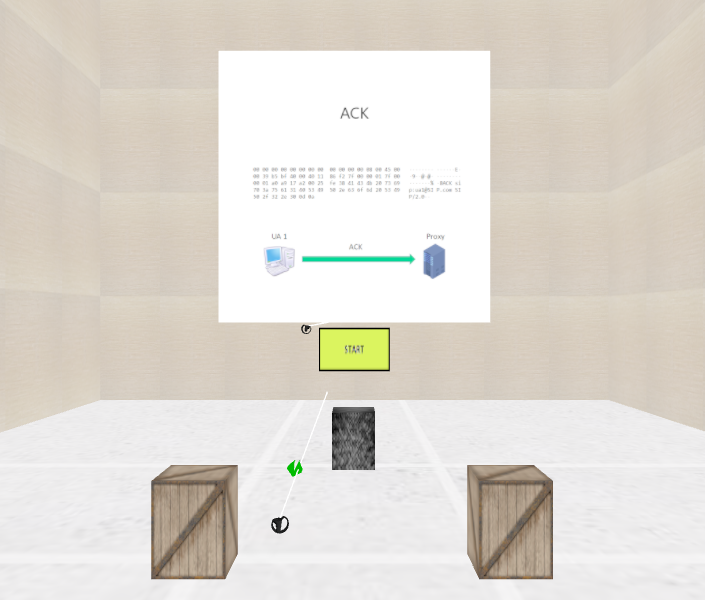
\includegraphics[width=12cm, keepaspectratio]{img/resultados/13-ACK.png}
  \caption{Reconocimiento ACK de UA1 completando el establecimiento de la llamada}
  \label{fig:13-ACK}
\end{figure}

% Bloque 4 %
\begin{figure}
  \centering
  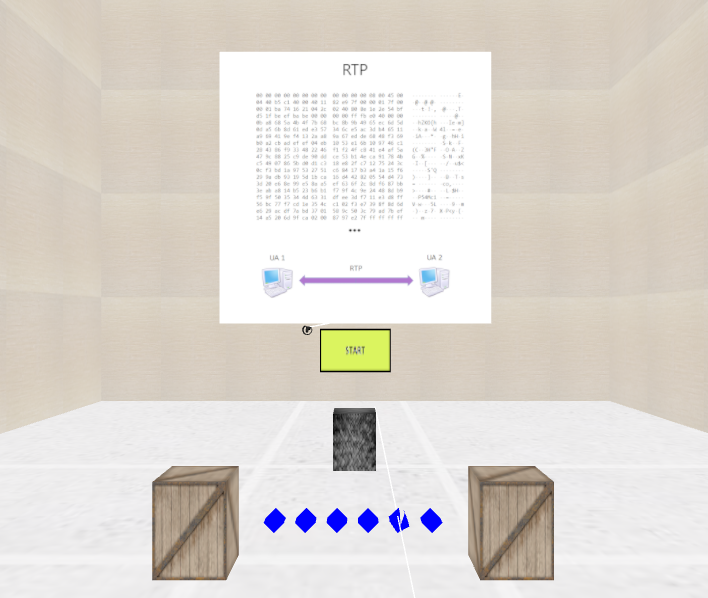
\includegraphics[width=12cm, keepaspectratio]{img/resultados/15-RTP.png}
  \caption{Transmisión de datos multimedia a través de paquetes RTP}
  \label{fig:15-RTP}
\end{figure}

\begin{figure}
  \centering
  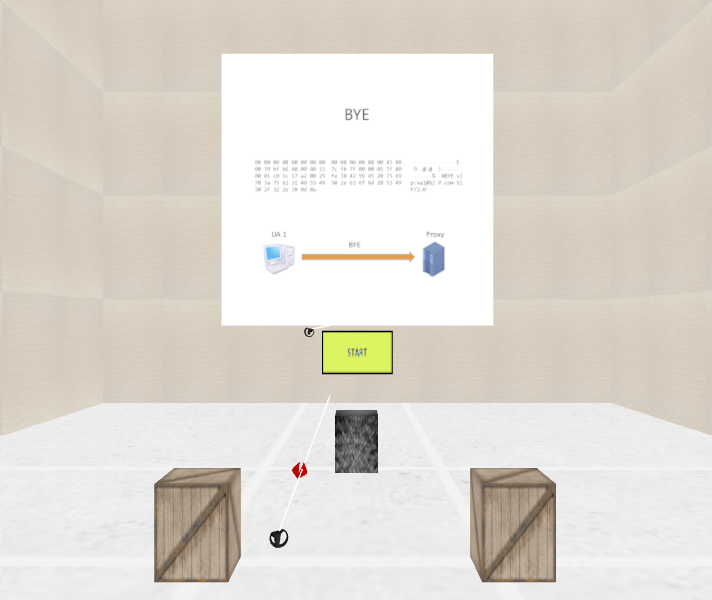
\includegraphics[width=12cm, keepaspectratio]{img/resultados/16-BYE.png}
  \caption{Mensaje BYE enviado para terminar la llamada}
  \label{fig:16-BYE}
\end{figure}

\begin{figure}
  \centering
  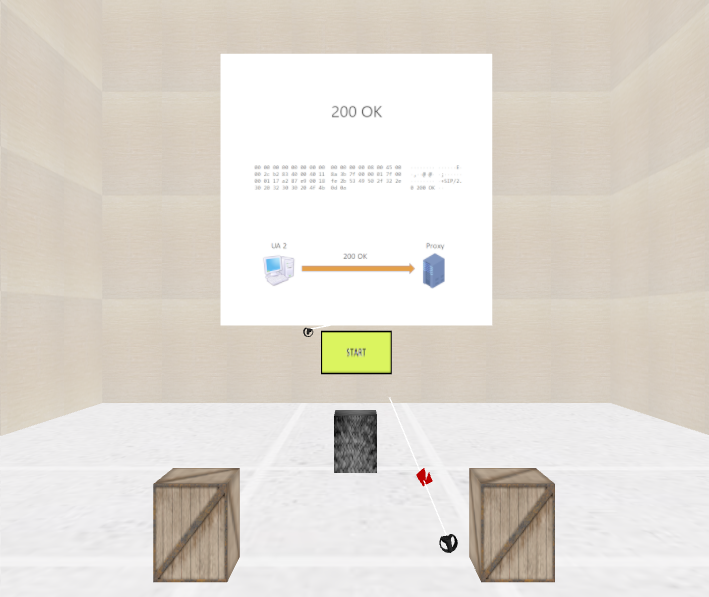
\includegraphics[width=12cm, keepaspectratio]{img/resultados/18-200OK.png}
  \caption{Confirmación del fin de la llamada con un 200 OK}
  \label{fig:18-200OK}
\end{figure}



%%%%%%%%%%%%%%%%%%%%%%%%%%%%%%%%%%%%%%%%%%%%%%%%%%%%%%%%%%%%%%%%%%%%%%%%%%%%%%%%
%%%%%%%%%%%%%%%%%%%%%%%%%%%%%%%%%%%%%%%%%%%%%%%%%%%%%%%%%%%%%%%%%%%%%%%%%%%%%%%%
% CONCLUSIONES %
%%%%%%%%%%%%%%%%%%%%%%%%%%%%%%%%%%%%%%%%%%%%%%%%%%%%%%%%%%%%%%%%%%%%%%%%%%%%%%%%

\cleardoublepage
\chapter{Conclusiones}
\label{chap:conclusiones}


\section{Consecución de objetivos}
\label{sec:consecucion-objetivos}

\subsection{Objetivo general}
El objetivo general del proyecto era construir una representación visual y funcional de los flujos de señalización y 
datos en un entorno de realidad virtual, utilizando tecnologías avanzadas como Three.js y módulos adicionales para facilitar 
la interacción en entornos VR. Este objetivo se ha cumplido satisfactoriamente, como se demostró en los resultados de funcionamiento 
del sistema, donde los usuarios pueden interactuar con la simulación de comunicaciones y experimentar de forma inmersiva el manejo de 
las comunicaciones en tiempo real.


\section{Aplicación de lo aprendido}
\label{sec:aplicacion}

A lo largo de mi formación en el grado de Ingeniería en Sistemas Audiovisuales y Multimedia, adquirí una serie de conocimientos y 
habilidades que han sido fundamentales para el desarrollo de mi proyecto de fin de grado. A continuación, detallo cómo se aplicaron 
específicamente algunas de las asignaturas más relevantes:

\begin{enumerate}
  \item \textbf{Informática I e Informática II:} Estas fueron las primeras asignaturas relacionadas con la programación, 
  las cuales sentaron las bases y aportaron los primeros pasos para desarrollar habilidades en el área de las telecomunicaciones.
  \item \textbf{Protocolos para la Transmisión de Audio y Vídeo por Internet:} Esta asignatura profundizó en la programación de manera 
  más específica, realizando prácticas que combinaban conocimientos técnicos con la utilización de protocolos de comunicación.
  \item \textbf{Construcción de Servicios y Aplicaciones Audiovisuales en Internet:} En esta asignatura se asentaron las bases del desarrollo 
  web utilizando lenguajes como JavaScript, HTML5 y CSS, elementos cruciales para la interfaz de usuario de mi proyecto.
  \item \textbf{Gráficos y Visualización en 3D:} Aprendí a desarrollar una parte significativa de mi proyecto, adquiriendo conocimientos en 
  gráficos 3D, conceptos básicos de WebGL y la creación de gráficos utilizando Three.js.
\end{enumerate}

En general, todas las asignaturas del grado han aportado valiosos conocimientos y fomentado el desarrollo del pensamiento crítico y la resolución de problemas, habilidades que he aplicado tanto en el TFG como en el entorno laboral.

\section{Lecciones aprendidas}
\label{sec:lecciones_aprendidas}

Durante el desarrollo de este proyecto, he adquirido una serie de conocimientos tanto técnicos como personales que han enriquecido 
mi experiencia y han contribuido a mi desarrollo profesional.

\begin{enumerate}
\item \textbf{Importancia de la planificación detallada:} Una de las lecciones más valiosas ha sido comprender la importancia de una planificación 
y organización en proyectos de desarrollo tecnológico.

\item \textbf{Profundización en tecnologías de realidad virtual:} El proyecto me permitió profundizar en el uso de tecnologías de realidad virtual, 
especialmente en la programación con JavaScript y el uso de bibliotecas como Three.js. Aprendí no solo a implementar estas tecnologías sino también 
a resolver problemas específicos relacionados con la renderización de gráficos 3D y la interactividad en entornos virtuales.

\item \textbf{Capacidad de adaptación y solución de problemas:} Desarrollo de la capacidad de buscar soluciones alternativas y adaptar el enfoque del proyecto según las 
circunstancias fue importante para el éxito del proyecto.

\item \textbf{Comprensión de los protocolos de comunicación:} El proyecto profundizó mi comprensión de los protocolos de comunicación como SIP y RTP. 
A través de la implementación práctica, pude ver cómo la teoría se aplica en situaciones reales.
\end{enumerate}


\section{Trabajos futuros}
\label{sec:trabajos_futuros}

Los resultados obtenidos implican que la aplicación de realidad virtual en el campo de las telecomunicaciones puede mejorar 
significativamente la comprensión de sistemas complejos de comunicación. Se recomienda que investigaciones futuras exploren 
ampliar la funcionalidad del sistema para incluir más escenarios de comunicación y evaluar su 
aplicabilidad en entornos educativos y profesionales.


%%%%%%%%%%%%%%%%%%%%%%%%%%%%%%%%%%%%%%%%%%%%%%%%%%%%%%%%%%%%%%%%%%%%%%%%%%%%%%%%
%%%%%%%%%%%%%%%%%%%%%%%%%%%%%%%%%%%%%%%%%%%%%%%%%%%%%%%%%%%%%%%%%%%%%%%%%%%%%%%%
% APÉNDICE(S) %
%%%%%%%%%%%%%%%%%%%%%%%%%%%%%%%%%%%%%%%%%%%%%%%%%%%%%%%%%%%%%%%%%%%%%%%%%%%%%%%%

\cleardoublepage
\appendix
\chapter{Manual de usuario}
\label{app:manual}

Esto es un apéndice.
Si has creado una aplicación, siempre viene bien tener un manual de usuario.
Pues ponlo aquí.

%%%%%%%%%%%%%%%%%%%%%%%%%%%%%%%%%%%%%%%%%%%%%%%%%%%%%%%%%%%%%%%%%%%%%%%%%%%%%%%%
%%%%%%%%%%%%%%%%%%%%%%%%%%%%%%%%%%%%%%%%%%%%%%%%%%%%%%%%%%%%%%%%%%%%%%%%%%%%%%%%
% BIBLIOGRAFIA %
%%%%%%%%%%%%%%%%%%%%%%%%%%%%%%%%%%%%%%%%%%%%%%%%%%%%%%%%%%%%%%%%%%%%%%%%%%%%%%%%

\cleardoublepage

% Las siguientes dos instrucciones es todo lo que necesitas
% para incluir las citas en la memoria
\bibliographystyle{abbrv}
\nocite{*}
\bibliography{memoria_JorgeGrande}  % memoria.bib es el nombre del fichero que contiene
% las referencias bibliográficas. Abre ese fichero y mira el formato que tiene,
% que se conoce como BibTeX. Hay muchos sitios que exportan referencias en
% formato BibTeX. Prueba a buscar en http://scholar.google.com por referencias
% y verás que lo puedes hacer de manera sencilla.
% Más información: 
% http://texblog.org/2014/04/22/using-google-scholar-to-download-bibtex-citations/

\end{document}
